\begin{frame}{}
    \begin{center}
        \LARGE Analisis
    \end{center}
\end{frame}


\begin{frame}{Estrategia del an\'alisis de datos}

\begin{itemize}
    \item El an\'alisis se basa en una selecci\'on de eventos a partir de una serie de variables experimentales las cuales buscan optimizar la eficiencia de la señal y reducir lo mas posible los procesos de ruido
    \item Recordar que en los datos experimentales solo se tiene informaci\'on de los muones reconstruidos y a partir de eso se infiere la posible producci\'on de fotones oscuros
    \item La selecci\'on de eventos se aplica a cada una de las muestras de simulaci\'on generadas y se estudia las eficiencias y distribuciones características 
\end{itemize}
    
\end{frame}


\begin{frame}{Secuencia del análisis de datos}

\begin{itemize}
    \item El análisis comienza con la muestra simulada (raw data) 
    \item Se procede a la selección de eventos, donde se reduce la cantidad de datos a analizar 
    \item Se procede a la obtención de resultados, gracias estadísticas y discusión de los mismos, algo similar al esquema mostrado en la figura 
\end{itemize}

\begin{figure}[h]
\centering
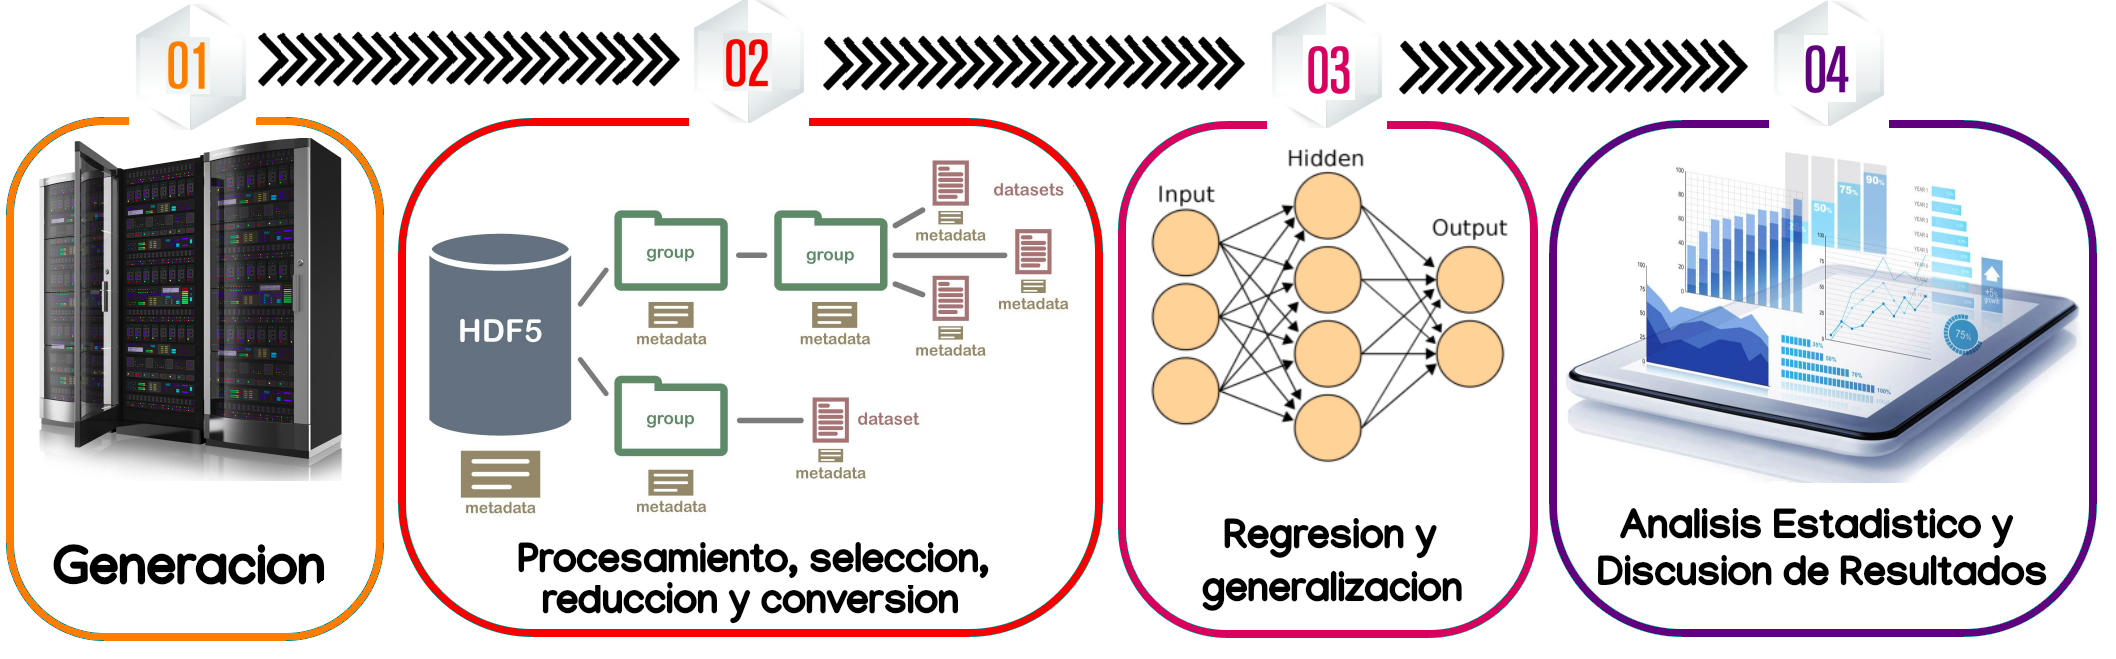
\includegraphics[width=0.8\textwidth]{Imag/procesos_darksusy.png}
\caption{Secuencia del análisis de datos}
\end{figure}

\end{frame}

\begin{frame}{Estructura del código de análisis}

\begin{itemize}
    \item Se desarrollo un entorno de simulaci\'on y an\'alisis de datos el cual esta basado en código de python y ROOT. 
    \item El entorno se encuentra hospedado en ACARUS y puede ser fácilmente extendido para el análisis de otros modelos (adicionales a Dark-SUSY)
\end{itemize}
    
\begin{figure}[h]
\centering
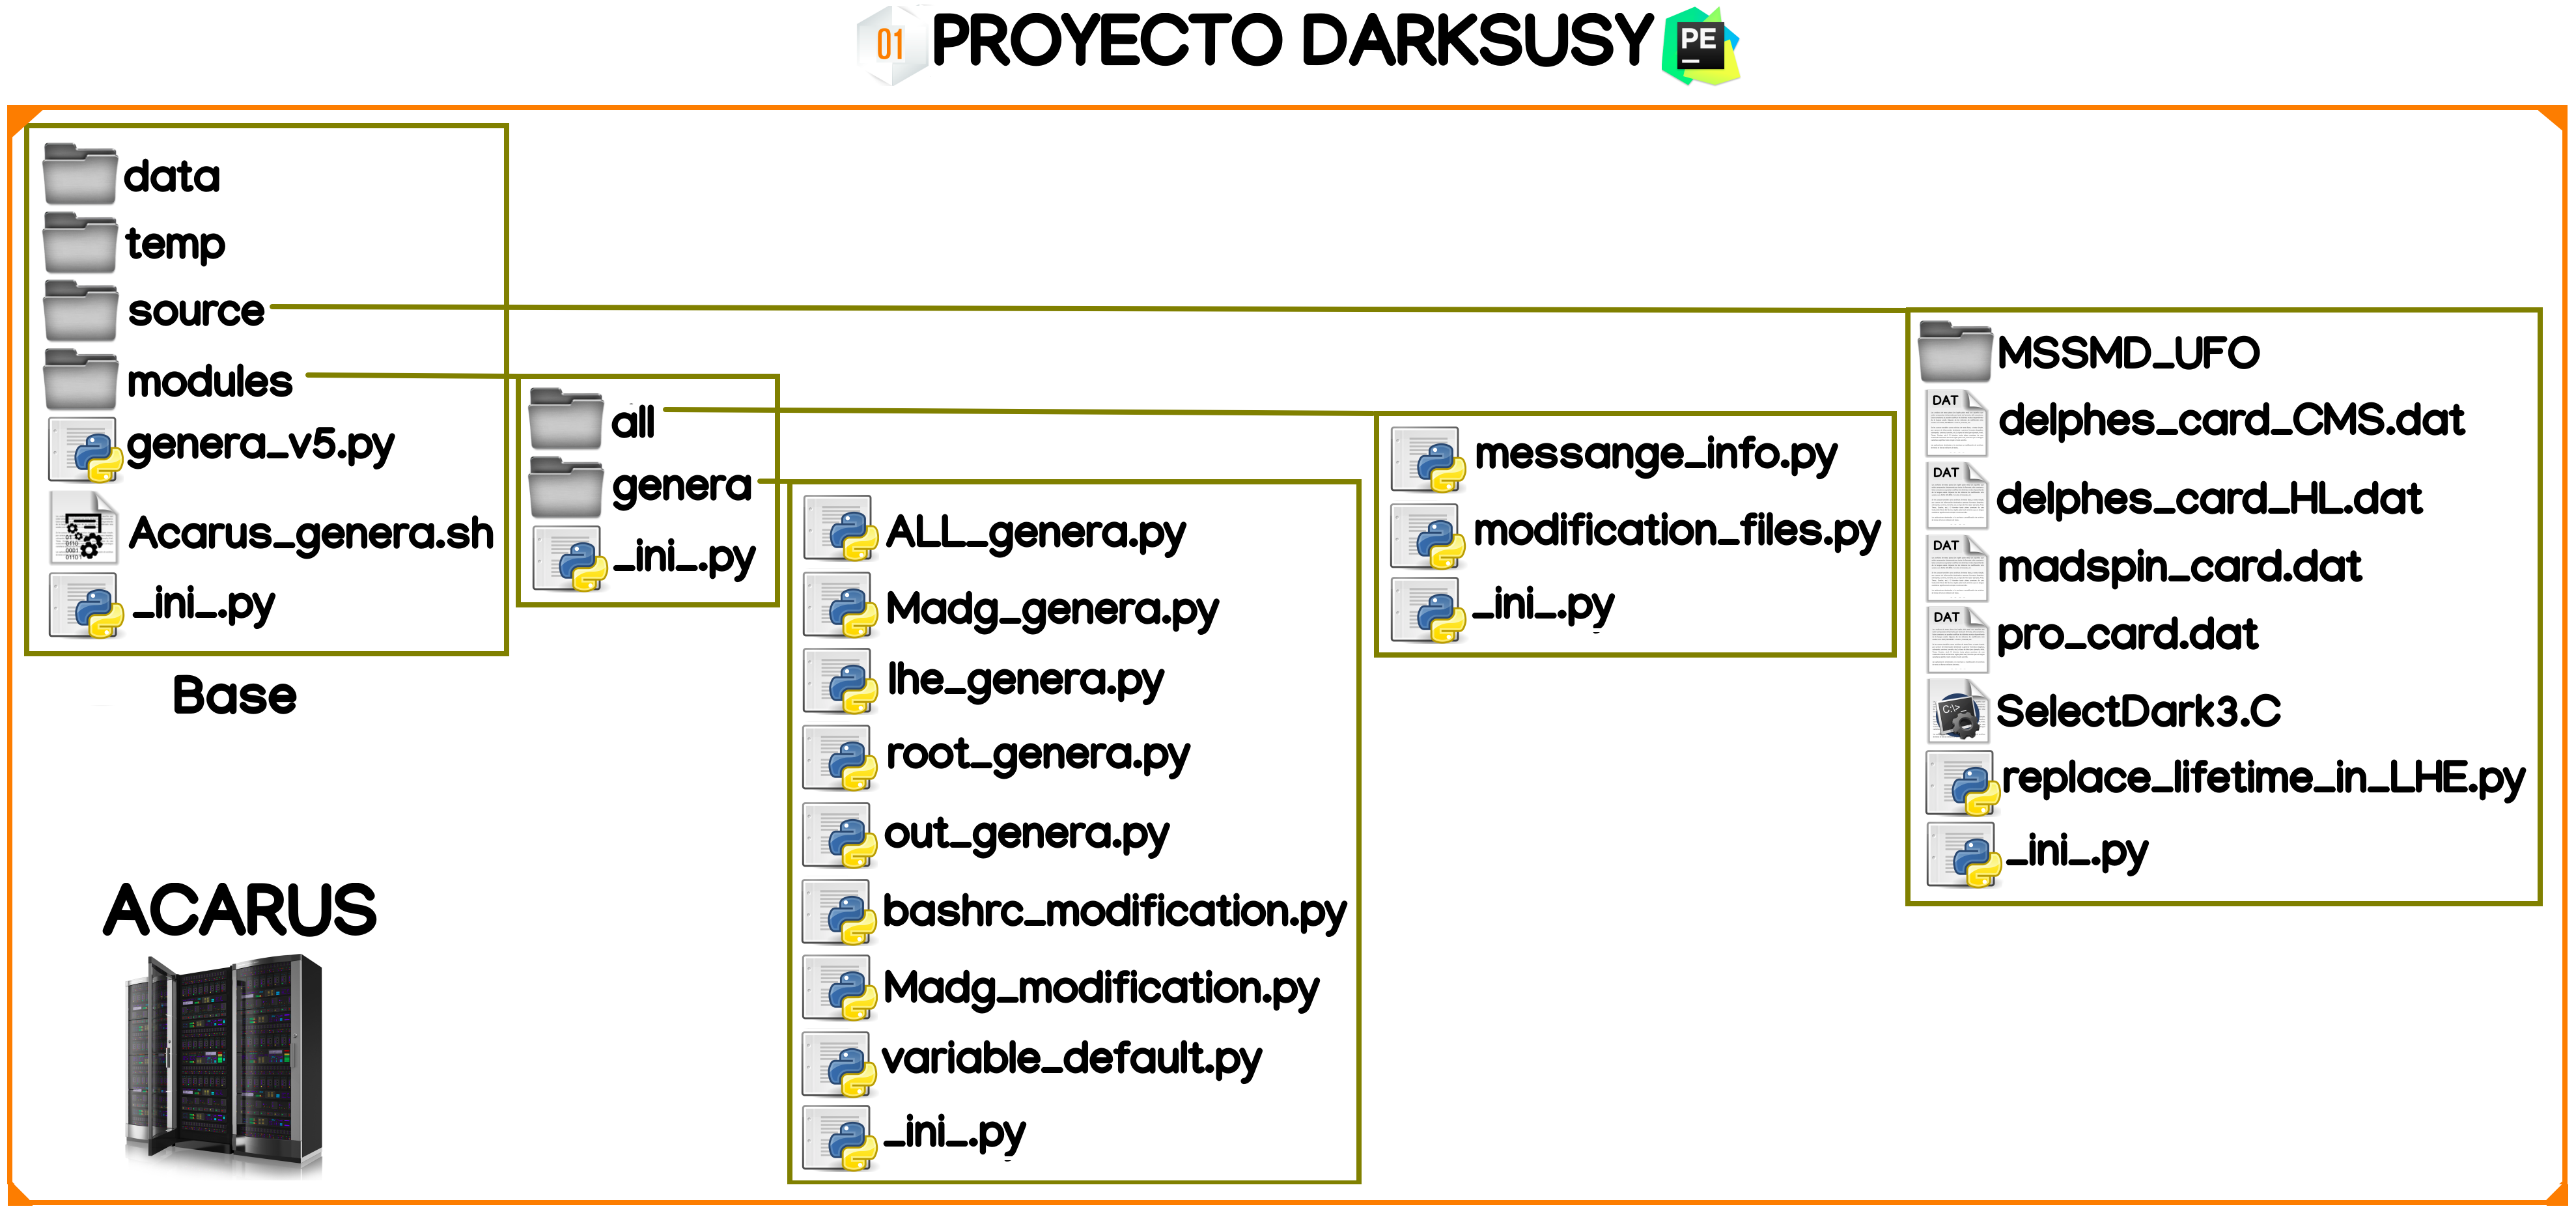
\includegraphics[width=0.8\textwidth]{Imag/proyecto_darksusy.png}
\caption{Estructura del código de análisis}
\end{figure}

\end{frame}



\begin{frame}{Selección preliminar}

\begin{itemize}
    \item \textbf{4$\mu$}: Selecci\'on de eventos con al menos 4 muones
    \begin{itemize}
        \item Muones con un momento transversal ($p_{T}$) mayor a
        \item Muones con un valor de pseudo-rapidez ($|\eta|$) menor a 2.4
    \end{itemize}
    \item \textbf{Algoritmo de pariamiento de muones}: Encontrar el par de muones optimos que con mayor probabilidad podrian ser generados por un foton oscuro
\end{itemize}
    
\end{frame}


\begin{frame}{Algoritmo de pariamiento de muones}
%\color{red} Francisco aqui incluir el diagrama de algoritmo de pariamiento
\begin{figure}[h]
\centering
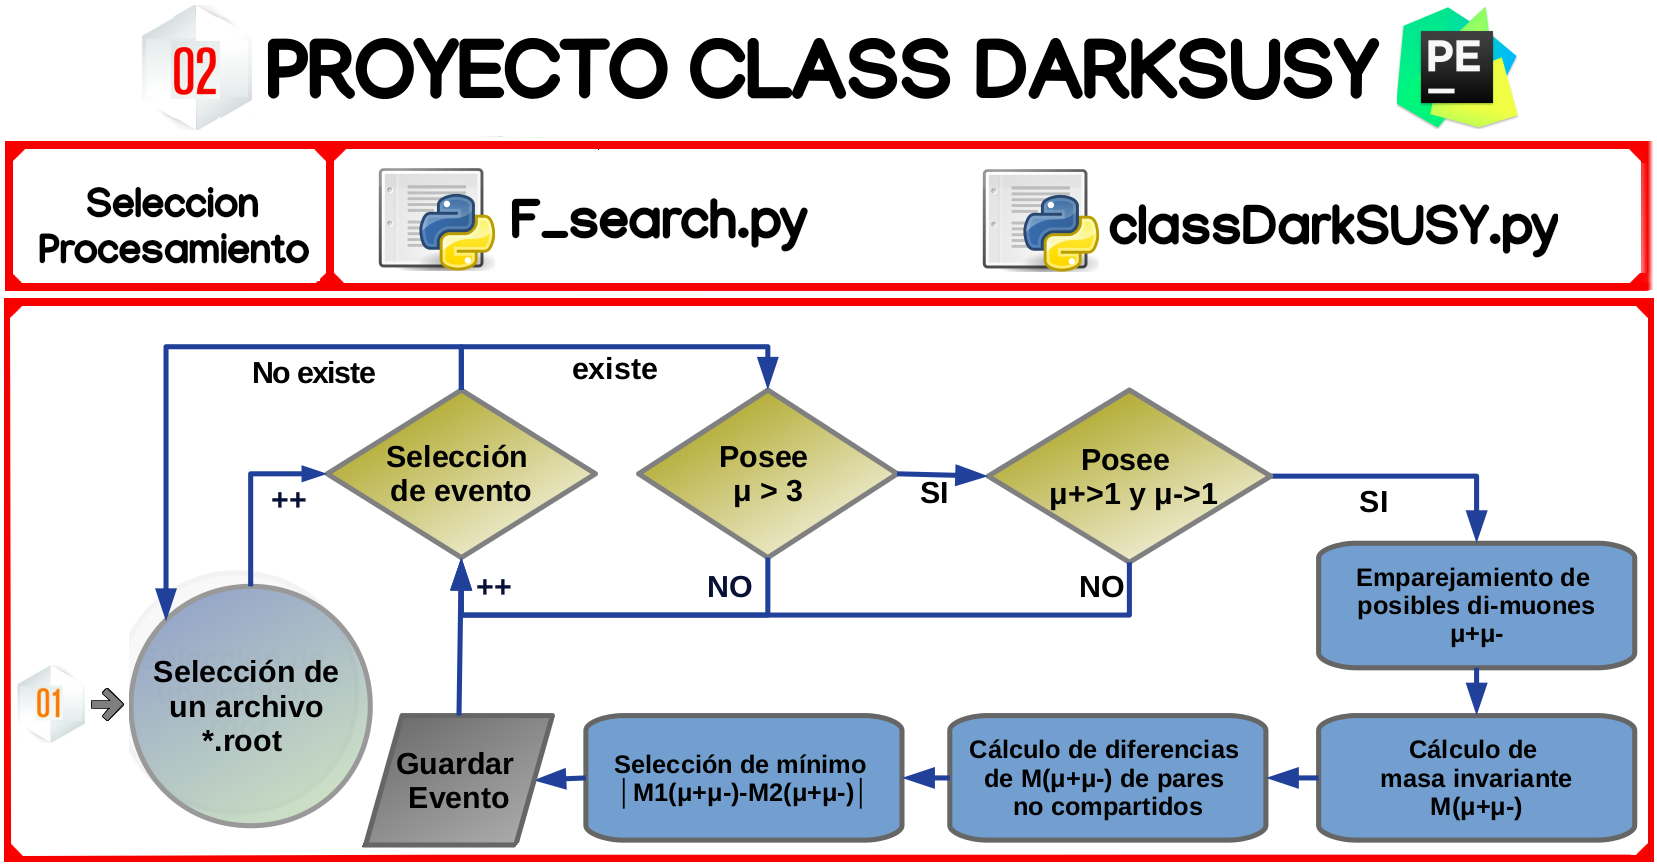
\includegraphics[width=1\textwidth]{Imag/class_darksusy.png}
\caption{Diagrama de algoritmo de pariamiento.}
\end{figure}   
\end{frame}

\begin{frame}{Eficiencia para fot\'on oscuro de baja masa}
\color{red} Francisco llenar estos numeros \color{black}
\begin{table}[]
    \centering
    \begin{tabular}{c|c|c|c|c|c|}
Selecci\'on  & $c\tau=XX$ & $c\tau=XX$ & $c\tau=XX$ & $c\tau=XX$ & $c\tau=XX$ \\  \hline
Sin corte         &  XXX & XXXX & XXXX & XXXX & XXX \\
4-$\mu$         &  XXX & XXXX & XXXX & XXXX & XXX \\
pariamiento    &  XXX & XXXX & XXXX & XXXX & XXX
     \end{tabular}
    \caption{Tabla con el numero de eventos despu\'es de cada selecci\'on $m_{\gamma_{D}}$=0.25 y diferentes valores del tiempo de vida}
    \label{tab:my_label}
\end{table}
    
\end{frame}

\begin{frame}{Eficiencias fot\'on oscuro de altas masa}
\color{red} Francisco llenar estos numeros \color{black}

\begin{table}[]
    \centering
    \begin{tabular}{c|c|c|c|c|c|}
Selecci\'on  & $c\tau=XX$ & $c\tau=XX$ & $c\tau=XX$ & $c\tau=XX$ & $c\tau=XX$ \\ \hline
Sin corte         &  XXX & XXXX & XXXX & XXXX & XXX \\
4-$\mu$         &  XXX & XXXX & XXXX & XXXX & XXX \\
pariamiento    &  XXX & XXXX & XXXX & XXXX & XXX
     \end{tabular}
    \caption{Tabla con el numero de eventos despu\'es de cada selecci\'on $m_{\gamma_{D}}$= 8~\GeV y diferentes valores del tiempo de vida}
    \label{tab:my_label}
\end{table}
    
\end{frame}


\begin{frame}{Distribuciones características: Masa invariante}
    
    \begin{itemize}
        \item Después de la selección preliminar se puede reconstruir la masa de los muones, dicha masa correspondería a la masa de los fotones oscuros. A continuación se muestra un ejemplo para los procesos con un valor esperado de $m_\gamma = 4 GeV$ :%\color{red} Francisco incluir estos gráficos 
    \end{itemize}
    
    \begin{figure}[ht]
    \centering
    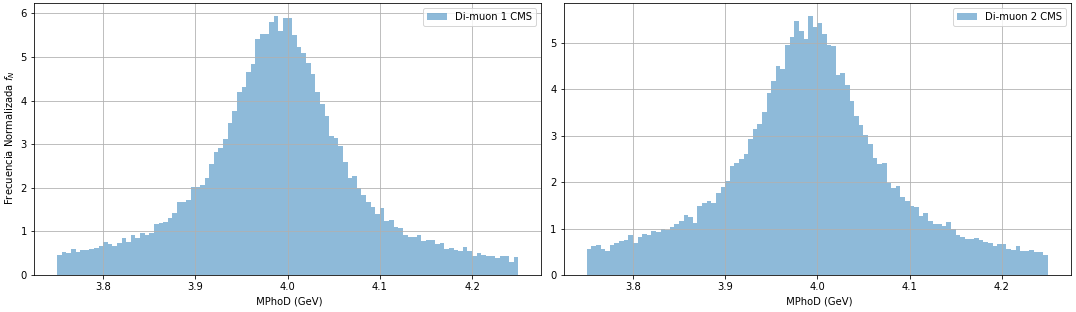
\includegraphics[width=1\textwidth]{Imag/Datos_Photon4muon_CORTE_CMS.png}
    \caption{Masa invariante para los di-muones.}
    \end{figure}
%    \begin{figure}[ht]
%        \begin{minipage}[b]{0.45\linewidth}
%            \centering
%            
\includegraphics[width=\textwidth]{placeholder.png}
%            \caption{Masa invariante primer di-muon}
%            \label{fig:a}
%        \end{minipage}
%        \hspace{0.5cm}
%        \begin{minipage}[b]{0.45\linewidth}
%            \centering
%            
\includegraphics[width=\textwidth]{placeholder.png}
%            \caption{Masa invariantes segundo di-muon}
%            \label{fig:b}
%        \end{minipage}
%    \end{figure}
\end{frame}

\begin{frame}{Distribuciones caracteristicas: Parametro de impacto (d0)}
    \color{red} Francisco incluir estos graficos (para el detector actual, todaviano no HL-LHC)
\end{frame}

\begin{frame}{}
    \begin{center}
        \LARGE High Luminosity LHC
    \end{center}
\end{frame}

\begin{frame}{Etapa de Alta luminosidad para el Gran Colisionador de Hadrones}
    \begin{itemize}
        \item El Gran Colisionador de Hadrones junto con sus experimentos principales estan en una etapa de actualizacion en preparacion para la etapa de alta luminosidad (2025-2035) 
        \item En particular para la deteccion de muones se instalaran una serie de nuevos detectores que ampliaran el rango de deteccion, muy en particular para la region de pseudo-rapidez ($2.4<|\eta|<3.0$) como se muestra en el la imagen
        \item Estos nuevos detectores permitiran la identificacion de muones en esta region, y aumentaran la probabilidad de detectar se\~nales como los fotones oscuros
    \end{itemize}
\end{frame}

\begin{frame}{Acutalizaci\'on del sistema de muones en el HL-LHC}

\begin{itemize}
    \item La actualizaci\'on de basa en la instalaci\'on de nuevos detectores de muones 
    \item Dicha detecci\'on amplia el rango de b\'usqueda para la posible detecci\'on de muones provenientes del fot\'on oscuro y otros modelos de fisica mas alla del modelo est\'andar
\end{itemize}

\begin{figure}
    \centering
    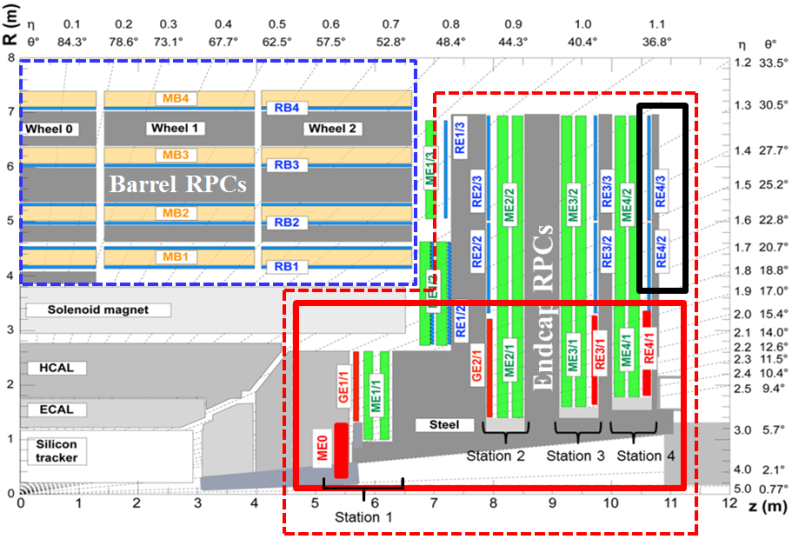
\includegraphics[width=1\textwidth]{muon_phase-2.png}
    \caption{Actualizacion del sistema de muones para la fase de alta luminosidad}
    \label{fig:my_label}
\end{figure}
    
\end{frame}


\begin{frame}{Comparacion distribuciones detector actual vs HL-LHC}
%\color{red} Francisco aqui poner distribucion de pseudorapidez comparando el detector actual y el detector nuevo
\begin{figure}
    \centering
    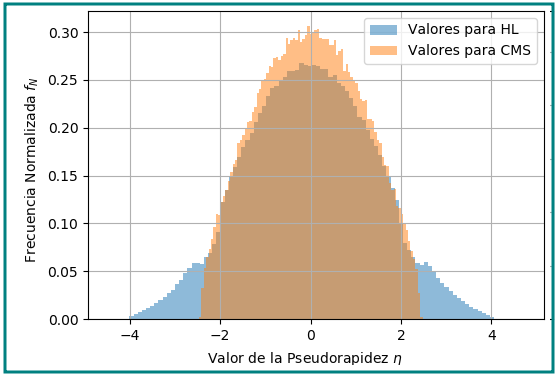
\includegraphics[width=1\textwidth]{Imag/Datos_Eta_ALL_simple.png}
    \caption{Comparar pseudorapidez.}
    \label{fig:my_label}
\end{figure}  
\end{frame}

\begin{frame}{Comparación de eficiencias detector actual vs HL-LHC.}
    
    \begin{itemize}
        \item Las ventajas de las actualizaciones se ve reflejada como una aumento en la eficiencia de la se\~nal
        \item La b\'usqueda del fot\'on oscuro durante el HL-LHC es uno de los objetivos fundamentales
    \end{itemize}
    
\begin{figure}[h]
\centering
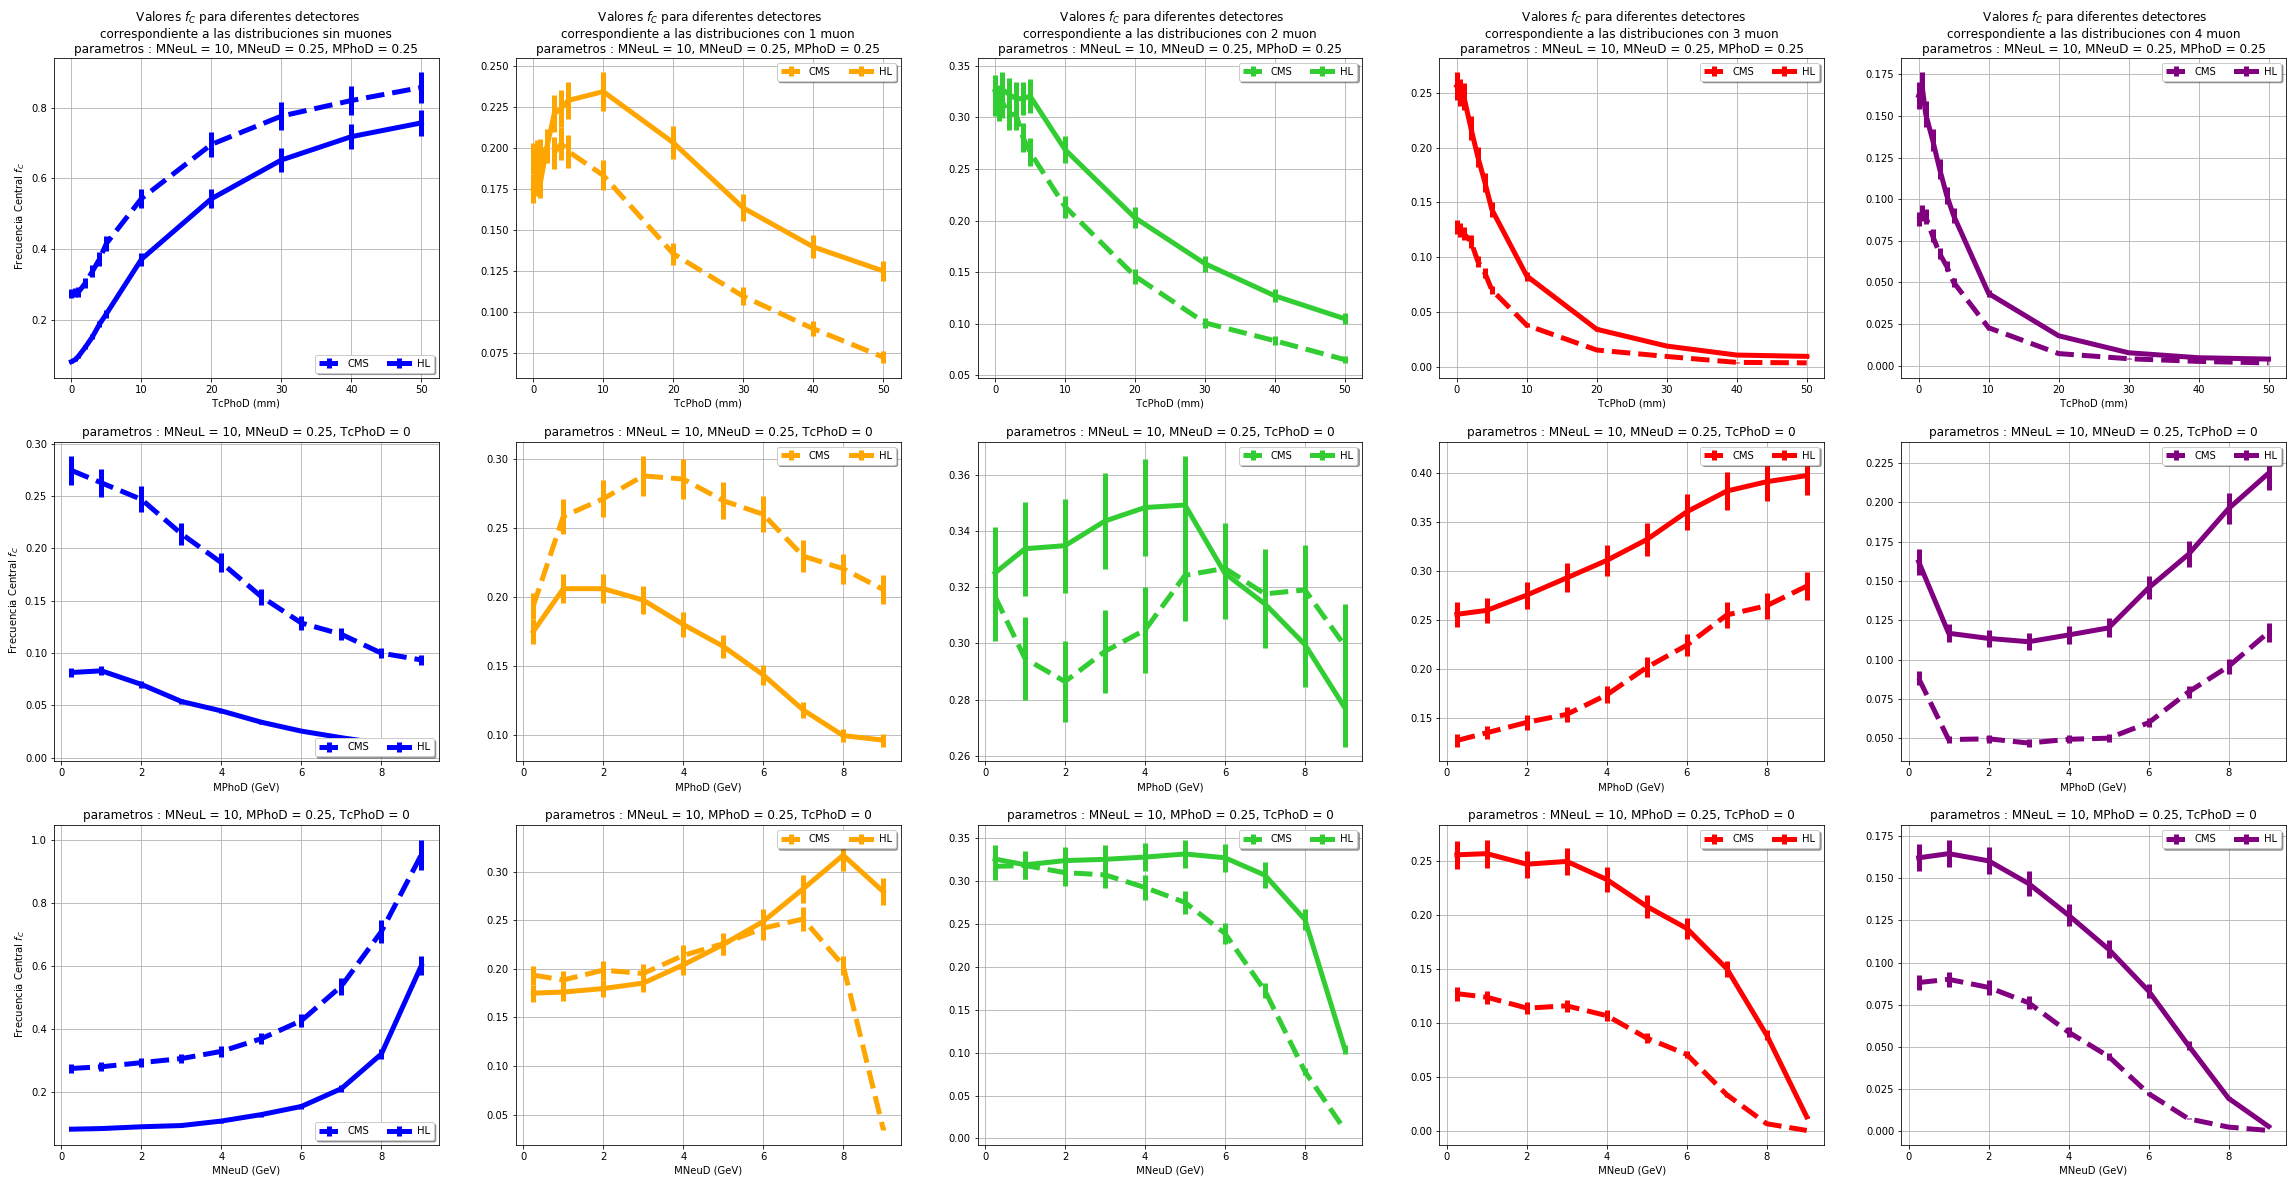
\includegraphics[width=0.8\textwidth]{Imag/Comparacion_Distribucion_Entries.png}
\caption{Comparacion de eficiencias del detector actual vs HL-LHC para las diferentes muestras}
\end{figure}

\end{frame}

\begin{frame}{Resumen}
\begin{itemize}
    \item Se integro el modelo Dark-SUSY en un entorno de simulacion
    \item Se desarrollo un entorno de simulaci\'on y an\'alisis el cual usa los recursos computacionales de la Universidad de Sonora (ACARUS) para generar resultados 
    \item Se estudio a detalle la se\~nal caracteristica de los fotones oscuros
    \item Se comparo la mejora en cuanto a eficiencia y rango de busqueda en la reconstruccion de muones del detector actual respecto a la actualizaci\'on en la etapa de alta luminosidad (HL-LHC) concluyendo que se tendra en general una mejor de \color{red} Francisco poner una estimacion de este numero XXX\% \color{black} de eficiencia en la b\'usqueda de esta se\~nal
\end{itemize}
    
\end{frame}


\begin{frame}{Siguientes Pasos}
\begin{itemize}
    \item Finalizar escritura de tesis (Finales de Junio) 
    \item Distribuir primer draft a  principios de Julio
    \tiem Presentar a finales de Julio o principios de Agosto
\end{itemize}
    
\end{frame}